%%%%%%%%%%%%%%%%%%%%%%%%%%%%%%%%%%%%%%%%%
% Programming/Coding Assignment
% LaTeX Template
%
% This template has been downloaded from:
% http://www.latextemplates.com
%
% Original author:
% Ted Pavlic (http://www.tedpavlic.com)
%
% Note:
% The \lipsum[#] commands throughout this template generate dummy text
% to fill the template out. These commands should all be removed when 
% writing assignment content.
%
% This template uses a Perl script as an example snippet of code, most other
% languages are also usable. Configure them in the "CODE INCLUSION 
% CONFIGURATION" section.
%
%%%%%%%%%%%%%%%%%%%%%%%%%%%%%%%%%%%%%%%%%

%----------------------------------------------------------------------------------------
%	PACKAGES AND OTHER DOCUMENT CONFIGURATIONS
%----------------------------------------------------------------------------------------

\documentclass{article}
\usepackage{fancyhdr} % Required for custom headers
\usepackage{lastpage} % Required to determine the last page for the footer
\usepackage{extramarks} % Required for headers and footers
\usepackage[usenames,dvipsnames]{color} % Required for custom colors
\usepackage{graphicx} % Required to insert images
\usepackage{caption}
\usepackage{listings} % Required for insertion of code
\usepackage{courier} % Required for the courier font
\usepackage{lipsum} % Used for inserting dummy 'Lorem ipsum' text into the template
\usepackage[colorlinks=true,linkcolor=black,anchorcolor=black,citecolor=black,menucolor=black,runcolor=black,urlcolor=black,bookmarks=true]{hyperref}
\usepackage[table,svgnames]{xcolor}
\usepackage{tabularx}
\usepackage{booktabs}
\usepackage{natbib}
\usepackage{pdfpages}

% Margins
\topmargin=-0.45in
\evensidemargin=0in
\oddsidemargin=0in
\textwidth=6.5in
\textheight=9.0in
\headsep=0.25in

\linespread{1.1} % Line spacing

% Set up the header and footer
\pagestyle{fancy}
\lhead{\hmwkAuthorName} % Top left header
\chead{\hmwkClass\ (\hmwkClassInstructor\ \hmwkClassTime): \hmwkTitle} % Top center head
\rhead{\firstxmark} % Top right header
\lfoot{\lastxmark} % Bottom left footer
\cfoot{} % Bottom center footer
\rfoot{Page\ \thepage\ of\ \protect\pageref{LastPage}} % Bottom right footer
\renewcommand\headrulewidth{0.4pt} % Size of the header rule
\renewcommand\footrulewidth{0.4pt} % Size of the footer rule

\setlength\parindent{0pt} % Removes all indentation from paragraphs

%----------------------------------------------------------------------------------------
%	CODE INCLUSION CONFIGURATION
%----------------------------------------------------------------------------------------

\definecolor{MyDarkGreen}{rgb}{0.0,0.4,0.0} % This is the color used for comments
\lstloadlanguages{Perl} % Load Perl syntax for listings, for a list of other languages supported see: ftp://ftp.tex.ac.uk/tex-archive/macros/latex/contrib/listings/listings.pdf
\lstset{language=Perl, % Use Perl in this example
        frame=single, % Single frame around code
        basicstyle=\small\ttfamily, % Use small true type font
        keywordstyle=[1]\color{Blue}\bf, % Perl functions bold and blue
        keywordstyle=[2]\color{Purple}, % Perl function arguments purple
        keywordstyle=[3]\color{Blue}\underbar, % Custom functions underlined and blue
        identifierstyle=, % Nothing special about identifiers                                         
        commentstyle=\usefont{T1}{pcr}{m}{sl}\color{MyDarkGreen}\small, % Comments small dark green courier font
        stringstyle=\color{Purple}, % Strings are purple
        showstringspaces=false, % Don't put marks in string spaces
        tabsize=5, % 5 spaces per tab
        %
        % Put standard Perl functions not included in the default language here
        morekeywords={rand},
        %
        % Put Perl function parameters here
        morekeywords=[2]{on, off, interp},
        %
        % Put user defined functions here
        morekeywords=[3]{test},
       	%
        morecomment=[l][\color{Blue}]{...}, % Line continuation (...) like blue comment
        numbers=left, % Line numbers on left
        firstnumber=1, % Line numbers start with line 1
        numberstyle=\tiny\color{Blue}, % Line numbers are blue and small
        stepnumber=5 % Line numbers go in steps of 5
}

% Creates a new command to include a perl script, the first parameter is the filename of the script (without .pl), the second parameter is the caption




%----------------------------------------------------------------------------------------
%	DOCUMENT STRUCTURE COMMANDS
%	Skip this unless you know what you're doing
%----------------------------------------------------------------------------------------

% Header and footer for when a page split occurs within a problem environment
\newcommand{\enterProblemHeader}[1]{
\nobreak\extramarks{#1}{#1 continued on next page\ldots}\nobreak
\nobreak\extramarks{#1 (continued)}{#1 continued on next page\ldots}\nobreak
}

% Header and footer for when a page split occurs between problem environments
\newcommand{\exitProblemHeader}[1]{
\nobreak\extramarks{#1 (continued)}{#1 continued on next page\ldots}\nobreak
\nobreak\extramarks{#1}{}\nobreak
}

\setcounter{secnumdepth}{0} % Removes default section numbers
\newcounter{homeworkProblemCounter} % Creates a counter to keep track of the number of problems

\newcommand{\homeworkProblemName}{}
\newenvironment{homeworkProblem}[1][Problem \arabic{homeworkProblemCounter}]{ % Makes a new environment called homeworkProblem which takes 1 argument (custom name) but the default is "Problem #"
\stepcounter{homeworkProblemCounter} % Increase counter for number of problems
\renewcommand{\homeworkProblemName}{#1} % Assign \homeworkProblemName the name of the problem
\section{\homeworkProblemName} % Make a section in the document with the custom problem count
\enterProblemHeader{\homeworkProblemName} % Header and footer within the environment
}{
\exitProblemHeader{\homeworkProblemName} % Header and footer after the environment
}

\newcommand{\problemAnswer}[1]{ % Defines the problem answer command with the content as the only argument
\noindent\framebox[\columnwidth][c]{\begin{minipage}{0.98\columnwidth}#1\end{minipage}} % Makes the box around the problem answer and puts the content inside
}

\newcommand{\homeworkSectionName}{}
\newenvironment{homeworkSection}[1]{ % New environment for sections within homework problems, takes 1 argument - the name of the section
\renewcommand{\homeworkSectionName}{#1} % Assign \homeworkSectionName to the name of the section from the environment argument
\subsection{\homeworkSectionName} % Make a subsection with the custom name of the subsection
\enterProblemHeader{\homeworkProblemName\ [\homeworkSectionName]} % Header and footer within the environment
}{
\enterProblemHeader{\homeworkProblemName} % Header and footer after the environment
}

%----------------------------------------------------------------------------------------
%	NAME AND CLASS SECTION
%----------------------------------------------------------------------------------------

\newcommand{\hmwkTitle}{A2} % Assignment title
\newcommand{\hmwkDueDate}{Saturday,\ October\ 14,\ 2017} % Due date
\newcommand{\hmwkClass}{\ INTRO. TO INFO RETRIEVAL:\ CS 734} % Course/class
\newcommand{\hmwkClassTime}{} % Class/lecture time
\newcommand{\hmwkClassInstructor}{Dr. Nelson} % Teacher/lecturer
\newcommand{\hmwkAuthorName}{Udochukwu Nweke} % Your name

%----------------------------------------------------------------------------------------
%	TITLE PAGE
%----------------------------------------------------------------------------------------

\title{
\vspace{2in}
\textmd{\textbf{\hmwkClass:\ \hmwkTitle}}\\
\normalsize\vspace{0.1in}\small{Due\ on\ \hmwkDueDate}\\
\vspace{0.1in}\large{\textit{\hmwkClassInstructor\ \hmwkClassTime}}
\vspace{3in}
}

\author{\textbf{\hmwkAuthorName}}
\date{} % Insert date here if you want it to appear below your name

%----------------------------------------------------------------------------------------

\begin{document}

\maketitle

%----------------------------------------------------------------------------------------
%	TABLE OF CONTENTS
%----------------------------------------------------------------------------------------

%\setcounter{tocdepth}{1} % Uncomment this line if you don't want subsections listed in the ToC

\newpage
\tableofcontents
\newpage

%----------------------------------------------------------------------------------------
%	PROBLEM 1
%----------------------------------------------------------------------------------------

% To have just one problem per page, simply put a \clearpage after each problem

\begin{homeworkProblem}


5.8 Write a program that can build a simple inverted index of a set of text documents.
Each inverted list will contain the file names of the documents that contain
that word.
Suppose the file A contains the text ``the quick brown fox'', and file B contains
``the slow blue fox''. The output of your program would be:\\

\% ./your-program A B\\
blue B\\
brown A\\
fox A B\\
quick A\\
slow B\\
the A B\\

\textbf{Solution 1:}\\
\lstinputlisting[caption=Inverted file code snippet, language=python]{P1.py}

In order to build a simple inverted index, I took the following steps:\\

1.  I read text from three or more different text files namely, A, B, and C. \\

2.  I generated a vocabulary by taking the union of all the terms in all the documents\\

3.  I stored the vocabulary into a dictionary with values as terms and keys as the files in which the terms occour in.  I generated an inverted index from the dictionary. This is demonstrated in listing 1, line 2-17.\\

 








 \end{homeworkProblem}
%----------------------------------------------------------------------------------------
% PROBLEM 2
%----------------------------------------------------------------------------------------


\begin{homeworkProblem}

4.8. Find the 10 Wikipedia documents with the most inlinks. Show the collection
of anchor text for those pages.\\ 

\textbf{Solution 2:}\\

\lstinputlisting[caption=Extract inlinks from wikismall, language=python]{P2.py}
 1.  I read the HTML files that were downloaded from the wiki small corpus from \url{http://www.searchengines-book.com}\\

 2.  I parsed the HTML files from step 1 to  \textit{BeautifulSoup} to extract outlinks. This is demonstrated in lisitng 2, \textit{getWikiOutlinks()} \\

 3.  I stored all the links extracted into a dictionary with key as link and value as the frequency of occurence of the link.\\

 4.  I sorted the dictionary by value in reverse order, as demonstrated in listing 2 line 115. \\

 5.  I picked the top 10 links that have the highest number of inlinks 
 

\end{homeworkProblem}

%----------------------------------------------------------------------------------------
% PROBLEM 3
%----------------------------------------------------------------------------------------


\begin{homeworkProblem}


4.1. Plot rank-frequency curves (using a log-log graph) for words and bigrams in
the Wikipedia collection available through the book website (\url{http://www.searchengines-book.com}).
Plot a curve for the combination of the two.What are the best
values for the parameter c for each curve?\\

\textbf{Solution 3:}\\

\lstinputlisting[caption= n-gram Vocabulary Code, language=python]{P3.py}
\lstinputlisting[caption=Extract link from wikismall, language=python]{n-gram.CSV}

\begin{figure}[h!]
 \centering
  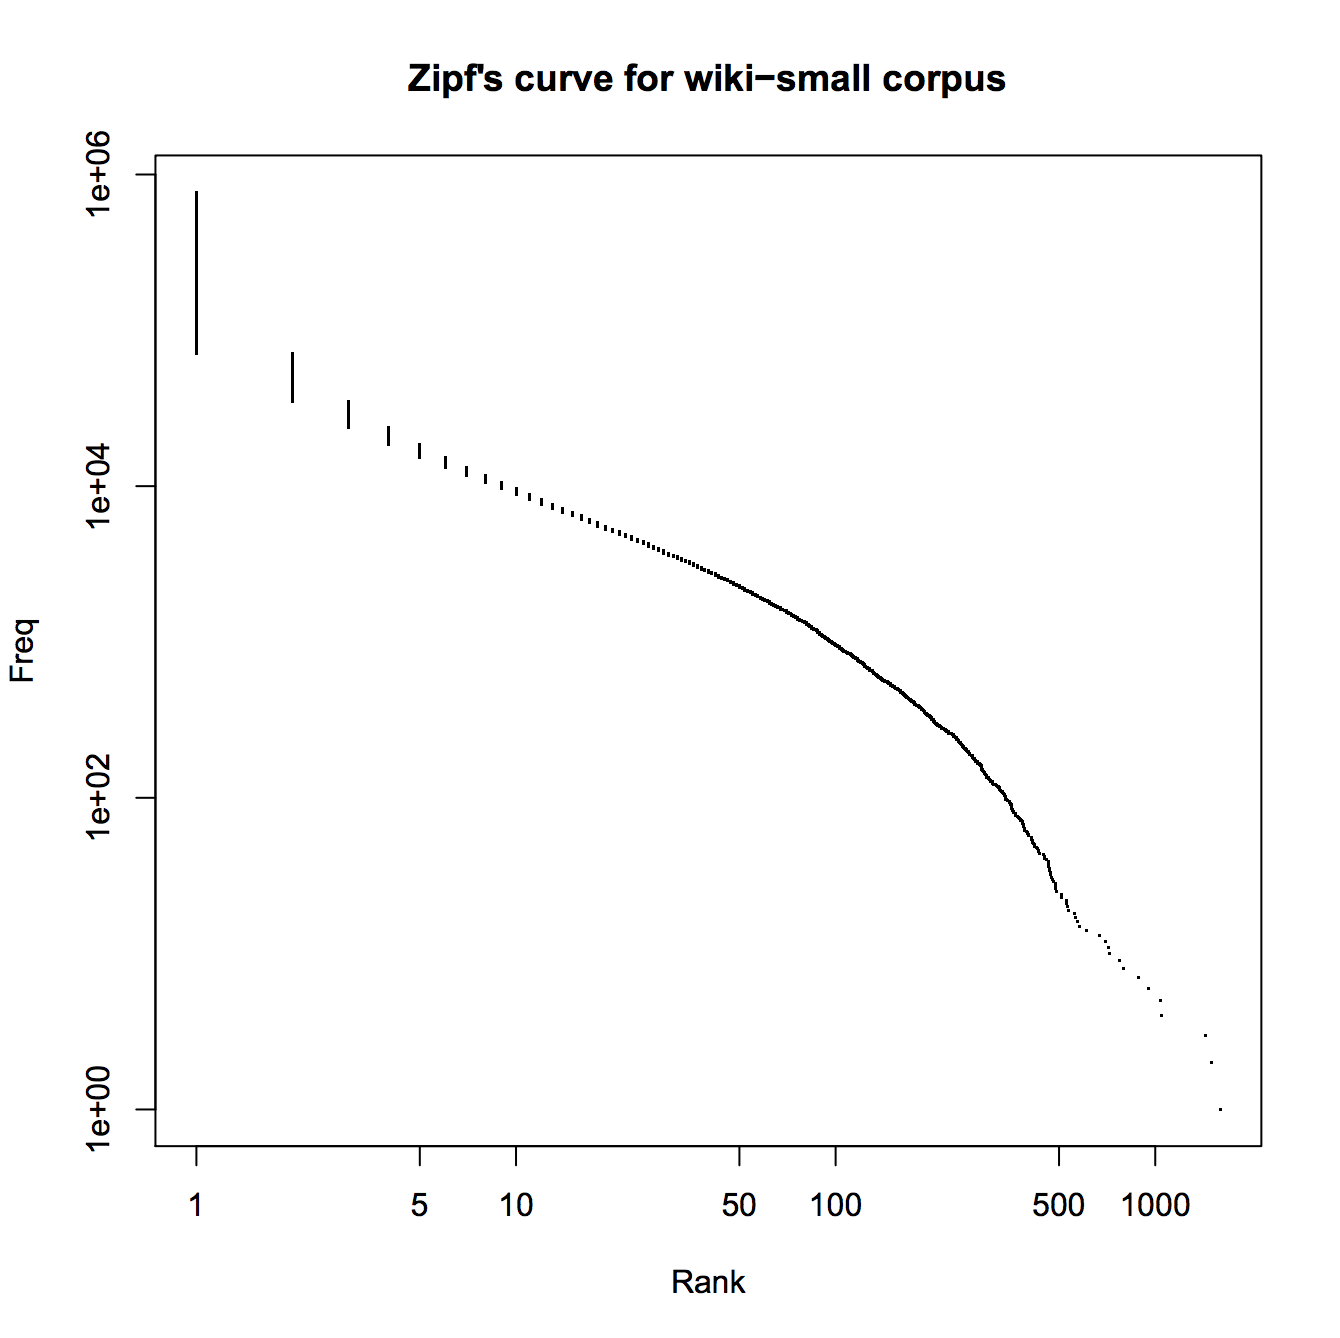
\includegraphics[width=0.5\textwidth]{Zipfs.png}
 \caption{Zipf's curve for n-grams}
  \label{fig:Zipf}
 \end{figure}

In order to plot rank-frequency for words and bigrams in in the wikipedia collection, I took the following steps: \\

1. I read the text files to get HTML text, this is demonstrated in line 35 of listing 3\\

2. I  used the \textit{boilerplate} removal library (Justext) to extract plain text.\\


3. I used sklearn \textit{CountVectorizer} to get 1 and 2-grams vocabulary. This is demonstrated in listing 3, line 41-47.\\

4. I stored the vocabulary (1-2 grams)  into a CSV file with. This is can be seen in listing 3.  \\

5. I plotted the \textit{1-2-grams.csv} with an Rscript and the graph is shown in Figure \ref{fig:Zipf}.\\

6. The best c values are 0.1 and 0.15. The graph in Figure \ref{fig:Zipf} shows that the frequently occuring c value lies where the graph goes on the horizontal line and that occurs half way between 0 and 0.2 which can be 0.1 and 0.15.

 

\end{homeworkProblem}

%----------------------------------------------------------------------------------------
% PROBLEM 4
%----------------------------------------------------------------------------------------

\begin{homeworkProblem}

4.2. Plot vocabulary growth for the Wikipedia collection and estimate the parameters
for Heaps’ law. Should the order in which the documents are processed
make any difference?\\

\textbf{Solution 4:}\\
\lstinputlisting[caption=Vocabulary growth, language=python]{P4.py}

\begin{figure}
 \centering
  \includegraphics[width=0.5\textwidth]{P4.png}
 \caption{Vocabulary Growth Plot}
  \label{Fig:Heap's curve}
 \end{figure}


 \begin{figure}
 \centering
  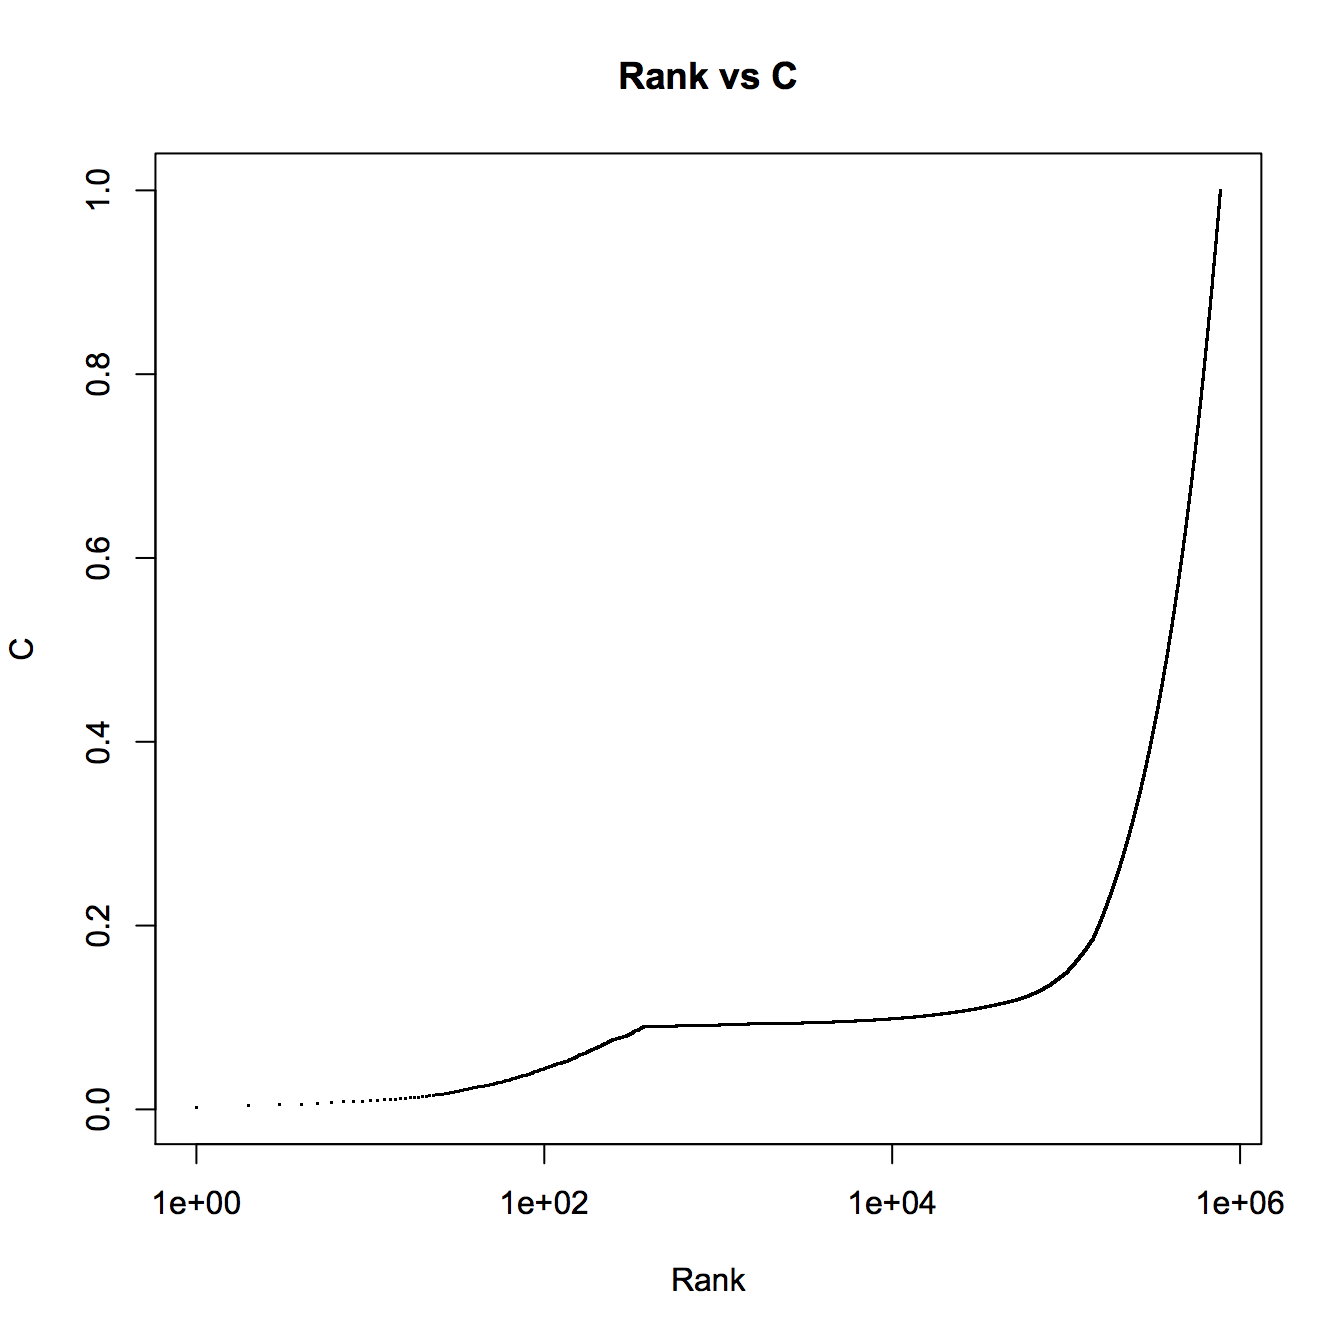
\includegraphics[width=0.5\textwidth]{RankVC.png}
 \caption{Heap's curve}
 \end{figure}

 
                               
1. The \textit{CountVectorizer} library is used to get the vocabulary which is a set of unique word, and the term frequency matrix. This is demonstrated in listing 5, line 24.\\

2. I kept accumulating the vocabulary by taking the union of the new vocabulary and the previous vocabulary from step 1. This is demonstrated in line 27, listing 5.\\

3. I used term frequency matrix to get the terms and the various frequencies and added it to get the word count as demonstrated in line 28, listing 5.\\

The order of documents processed does not make any difference because the order did not affect the size of the corpus.  `` Heaps’ law predicts that the number of new words will increase very rapidly when the corpus is small and will continue to increase indefinitely, but at a slower rate for larger corpora''. It is size of the vocabulary that will have an effect .\\

The Heap's k and beta parameters shows that Heap's law is a good fit.

Estimated Heap’s law parameters : k = 0.90 and beta = 0.009. \\

The vocabulary growth plot for Heap's law in Figure \ref{Fig:Heap's curve} shows that Heap's is a good fit with the estimated k and beta parameters




 

\end{homeworkProblem}
%----------------------------------------------------------------------------------------
% PROBLEM 5
%----------------------------------------------------------------------------------------

\begin{homeworkProblem}

4.6. Process five Wikipedia documents using the Porter stemmer and the Krovetz
stemmer. Compare the number of stems produced and find 10 examples of differences
in the stemming that could have an impact on ranking

\textbf{Solution 5:}\\

\lstinputlisting[caption= Port and Krovetz stemming, language=python]{P5.py}

1.  I read the text files to get HTML text.\\

2.  I  used the \textit{boilerplate} removal library (Justext) to extract plain text.\\


3. I applied Porter and Krovetz stemmers to plain text of five documents from \textit{wiki-small-files.txt}; this is demonstrated in listing 6, and the result is saved in wikiDoc1.txt, wikiDoc2.txt, wikiDoc3.txt, wikiDoc4.txt and wikiDoc5.txt.\\


4. I compared the output of Krovetz and Porter stemmers for the following 10 examples\\


 \begin{table}[h!]
 \centering
 \caption{Stemming Comparison}
  \label{tab:stem}
  \begin{tabular}{ | l | l | l|}
  \hline
 Original Word & PorterStemmer Result&KrovetzStemmer Result\\
 \hline
 Archives & archiv & archives\\
 \hline
 Dublirer & dublir& dublirer\\
 \hline
 Federal & feder & federal\\
 \hline
 studied & studi & studied \\
 \hline
 Her husband was Robert Dublirer & her husband wa robert dublir &her husband was robert dublirer\\
 \hline
 Arts Project&art project&  arts project \\
 \hline
 encyclopediaDorothy & encyclopediadorothi & encyclopediadorothy\\
 \hline
 Aristodemos & aristodemo  & aristodemos \\
 \hline
 Aristodemos Kaldis  & aristodemo kaldi & aristodemos kaldis \\
 \hline
 Art Students League & art student leagu & art students league \\
 \hline

  \end{tabular}
  \end{table}

From the stemmed result in Table \ref{tab:stem}, Krovetz returned almost the same word as the original words. The result is meaningful and can be use as a query. Krovetz doesn't have so much impact on ranking.\\

Porter stem results are almost not English words. Most of the results cannot be identified with the original word. This will have impact on ranking. Krovetz will produce a better ranking.\\

From the example in Table \ref{tab:stem}, it Porter have more stemmed words than Krovetz.



\end{homeworkProblem}

\nocite{*}
\bibliographystyle{plain}
\bibliography{A2Ref}

\end{document}